% ICASSP official spconf layout: four technical pages and one references page.
\documentclass{article}
\usepackage{spconf,amsmath,amssymb,amsthm,booktabs,graphicx}
\usepackage{tikz}
\usetikzlibrary{arrows.meta,positioning}
\usepackage[hidelinks]{hyperref}
\renewcommand{\rmdefault}{lmr}
\newcommand{\RACF}{\textsc{RACF}}
\newcommand{\TV}{d_{\mathrm{TV}}}
\newcommand{\score}{S}
\newtheorem{theorem}{Theorem}
\newtheorem{proposition}{Proposition}
\newcommand{\AuthorName}{Zelin LI}
\newcommand{\AuthorAffiliation}{Affiliation and e-mail to be completed before submission}
\begin{document}
\ninept
\title{Residual-Aware Conformal Action Filtering for Offline Reinforcement Learning in Adaptive Cruise Control}
\name{\AuthorName}
\address{\AuthorAffiliation}
\maketitle
\begin{abstract}
Deploying an offline reinforcement learning policy under changed vehicle
dynamics requires reconciling constraint satisfaction with the policy's
control objective. We present residual-aware conformal action filtering
(RACF), which combines calibrated prediction residuals, a finite dynamics
ensemble, and constrained action correction. A score-level total-variation
bound characterizes one-step coverage, while an episode-maximum construction
extends the residual analysis to finite horizons. In paired adaptive cruise
control evaluations with 12 policies and four operating conditions, static,
adaptive, and fixed-envelope filters increase episode-safe rates from
41.7\% to 88.9\%, 94.3\%, and 95.3\%, respectively. All filtered policies
complete the 500-step horizon without collision. Analysis of shared reset
trials reveals policy-dependent gains and a measurable comfort cost.
These results identify residual calibration and candidate selection as
complementary tools for deploying frozen policies under dynamics variation.
\end{abstract}
\begin{keywords}
Conformal prediction, offline reinforcement learning, safety filtering,
adaptive cruise control, distribution shift.
\end{keywords}
\section{Introduction}
Offline reinforcement learning (RL) offers a practical route to vehicle
control from previously collected driving data \cite{levine2020offline}.
Algorithms such as implicit Q-learning (IQL) and conservative Q-learning
(CQL) address action-distribution mismatch during policy training
\cite{kostrikov2022iql,kumar2020cql}. Recent cross-domain offline RL also
trains policies for test-time dynamics perturbations \cite{qiao2026droco}.
Deployment nevertheless introduces a second source of mismatch: a frozen
policy encounters vehicle mass, road grade, and actuation
characteristics that differ from those represented by its training data.
In adaptive cruise control (ACC), these changes affect braking response and
the distance required to maintain a prescribed time headway. A useful
deployment mechanism must therefore correct unsafe commands while retaining
the policy's tracking behavior.

Safe RL methods address this problem through constrained learning or runtime
intervention \cite{brunke2022safe}.
Shielding and safety layers act directly on proposed commands
\cite{alshiekh2018shielding,dalal2018safe}; control barrier functions and
predictive safety filters connect these corrections to model-based
constraints \cite{ames2017cbf,wabersich2021psf}.
Learning-based model predictive control (MPC) captures the interaction
between estimation error and constrained decision making
\cite{aswani2013lbmpc}. For a frozen RL policy, the central
design question is how a data-calibrated model-error margin should influence
the amount of action intervention.

Conformal prediction provides finite-sample prediction regions from held-out
residuals \cite{vovk2005algorithmic,angelopoulos2023gentle}. Work on
covariate shift, non-exchangeability, and robust validation characterizes
how those regions change under distribution mismatch
\cite{tibshirani2019covariate,barber2023beyond,cauchois2024robust}.
Conformal planning and adaptive conformal control embed uncertainty regions
in dynamic constraints \cite{lindemann2023safeplanning,zhou2024safetycritical}.
Robust conformal runtime verification explicitly models design-to-deployment
trajectory shift \cite{zhao2024robuststl}.
Recent work also couples conformal temporal-logic monitoring with RL
shielding \cite{beirami2026} and uses generative priors to recalibrate
planning under changing environments \cite{rahaman2026shift}.
We study this residual-to-action interface across frozen policy families
and explicit physical perturbations.

We develop residual-aware conformal action filtering (RACF) as a post-policy
deployment layer for this setting.
RACF combines a fixed prediction model, a calibrated residual threshold, and
robust projection over a finite set of dynamics hypotheses. Its adaptive
variant uses observed residuals to select relevant hypotheses; a fixed
episode-envelope variant changes the margin at which the policy is filtered.
The specific contribution is their common, auditable interface for frozen
offline policies. We provide a
score-shift coverage analysis with a finite-horizon extension, and a paired
evaluation of 12 policies under four ACC operating conditions. The resulting
evidence quantifies both constraint improvement and intervention cost, and
identifies where policy behavior and model uncertainty interact.

\section{Problem Formulation}
Consider a finite-horizon controlled process with observation $o_t$ and
frozen policy $a_t^\pi=\pi(o_t)$. We seek an applied action $a_t$ in a bounded set
$\mathcal A$ that preserves a safety margin $h(s_{t+1})\geq0$ and stays
close to $a_t^\pi$. The policy is trained before calibration and evaluation.
The deployment filter changes its actions without updating policy weights.

The ACC state is $s=(v_e,v_l,g,v_d,\phi)$, comprising ego speed, lead
speed, inter-vehicle gap, desired speed, and grade. We linearly normalize a
protocol-defined actuator interval $[F_{\min},F_{\max}]=[-6000,4000]$ N:
$F(a)=F_{\min}+(a+1)(F_{\max}-F_{\min})/2=-1000+5000a$ N for
$a\in[-1,1]$. Under a gain shift $\gamma$, the simulator applies
$F_\gamma(a)=-1000+5000\gamma a$ N. These bounds specify the experiment;
the linear normalization is the policy--actuator interface. With sampling interval
$\Delta t=0.1$ s, longitudinal prediction uses drag, rolling resistance,
grade, and a mass-dependent acceleration \cite{rajamani2012vehicle}.
The nominal model $f_0$ approximates these effects and predicts constant lead
speed. Model hypotheses $f_\theta$ vary mass, grade, and actuator gain over
a finite set $\Theta$.

We use the constant-time-headway (CTH) spacing policy
$d_{\mathrm{CTH}}=d_0+T_hv_e$, a standard ACC design
\cite{wu2020spacing,molnar2023cruise}. Our protocol fixes
$d_0=3$ m, $T_h=1.5$ s, and $v_{\max}=30$ m/s, giving
\begin{equation}
 h_{\mathrm{CTH}}(s)=\min\{g-d_0-T_hv_e,\;v_{\max}-v_e\}.
 \label{eq:margin}
\end{equation}
The margin changes with $g$ and $v_e$, while its three protocol coefficients
remain fixed. Closing-speed and braking-distance alternatives such as
time-to-conflict and responsibility-sensitive safety (RSS) represent a richer
dynamic risk model \cite{molnar2023cruise,shalevshwartz2017rss}.
For the Euclidean norm in these physical coordinates,
$h_{\mathrm{CTH}}$ is Lipschitz with
$L_h=\sqrt{1+T_h^2}=\sqrt{3.25}$.
Calibration and evaluation use the same physical coordinates; changing their
scaling requires recalibrating the score and its Lipschitz conversion.

The episode endpoint monitors the same time-headway flag $g<3+1.5v_e$;
collision, violation duration, tracking error, and comfort provide
complementary outcomes.

\section{RACF Method}
\subsection{Calibration and robust action correction}
For an independently collected transition $Z=(s,a,s^+)$, define the fixed
nominal-model score $S(Z)=\|s^+-f_0(s,a)\|_2$. Given $n$ calibration
scores, let
\begin{equation}
 k=\lceil(n+1)(1-\alpha)\rceil,\qquad q_\alpha=S_{(k)},
 \label{eq:quantile}
\end{equation}
where $S_{(k)}$ is the order statistic and $q_\alpha=+\infty$ if $k>n$.
Conformal risk control offers a broader loss construction
\cite{angelopoulos2024crc}; a residual norm makes our
margin-to-control conversion explicit.

At each step, RACF constructs the feasible set
\begin{equation}
 \mathcal F_t(m_t)=\{a\in\mathcal A:
       h(f_\theta(s_t,a))\geq m_t,\;\theta\in\Theta_t\}
 \label{eq:feasible}
\end{equation}
and computes
\begin{equation}
 a_t=\arg\min_{a\in\mathcal F_t(m_t)}\|a-a_t^\pi\|_2^2.
 \label{eq:projection}
\end{equation}
The candidate set is a local protocol object, generated before evaluation;
runtime control reads no external dataset or service. In the main study,
$\Theta=\{1500,1800\}\!\times\!\{0,3\}\!\times\!\{0.7,1.0\}$
contains eight mass (kg), grade (degrees), and actuator-gain hypotheses.
The combined 1800 kg/$2^\circ$ condition is an interpolation stress cell,
not an exact member of this grid.
Static RACF sets $\Theta_t=\Theta$ and $m_t=\eta q_\alpha$.
The coefficient $\eta$ specifies the operating margin; the analytical
residual-to-safety conversion uses $\eta\geq L_h$.
When the feasible set is empty or the solver fails its feasibility check,
the controller applies bounded maximum braking and records a fallback.
This makes feasibility, intervention, and realized safety independently
observable.

\begin{figure}[t]
\centering
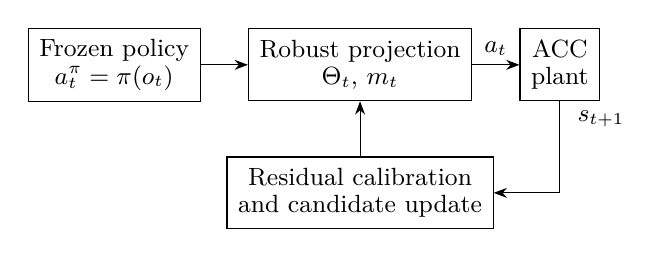
\begin{tikzpicture}[>=Stealth, font=\fontsize{9}{10}\selectfont,
 node distance=5mm, box/.style={draw,align=center,inner sep=4pt,minimum height=9mm}]
 \node[box] (policy) {Frozen policy\\$a_t^\pi=\pi(o_t)$};
 \node[box,right=6mm of policy] (filter) {Robust projection\\$\Theta_t,\,m_t$};
 \node[box,right=6mm of filter] (plant) {ACC\\plant};
 \draw[->] (policy) -- (filter);
 \draw[->] (filter) -- node[above] {$a_t$} (plant);
 \node[box,below=7mm of filter] (cal) {Residual calibration\\and candidate update};
 \draw[->] (cal) -- (filter);
 \draw[->] (plant.south) |- (cal.east);
 \node[right=1mm of plant.south,anchor=north west] {$s_{t+1}$};
\end{tikzpicture}
\caption{RACF combines a frozen policy with calibrated action correction.
The transition observed after execution updates the next control step.}
\label{fig:method}
\end{figure}

\subsection{Adaptive selection and horizon-aware envelopes}
The adaptive variant ranks each candidate by the residual quantile in a
40-transition window, evaluated every ten steps after twenty observations.
It retains at most four candidates with the smallest residual scores.
Observed grade further restricts candidates within $0.75^\circ$ of a grid
value; intermediate grades retain the available grid. A residual trigger
reopens the full candidate set for a bounded recovery period. The threshold
uses a separate 100-transition window with its calibration value as a floor.
All updates consume the transition just completed, so the action at time
$t$ uses information available before its execution (Fig.~\ref{fig:method}).
This empirical adaptation complements the explicit online coverage objectives
studied in adaptive conformal inference \cite{gibbs2021adaptive}.

A horizon-aware alternative calibrates the maximum score of a complete
episode $\tau$:
\begin{equation}
 M_H(\tau)=\max_{0\leq t<H} S(Z_t).
 \label{eq:maxscore}
\end{equation}
Applying~\eqref{eq:quantile} to independent episode maxima yields an
envelope $q_H$. The evaluated fixed-envelope variant instead transfers the
previously selected threshold $B=0.45$ to the 12-policy study. This tests the
effect of an episode-oriented operating margin across policies; the formal
max-score result below describes calibration on complete episodes.

\section{Coverage and Control Implications}
\subsection{Coverage under score-distribution shift}
Let $P$ be the calibration score law and $Q$ the test score law. The model
and score function are fixed before collecting calibration data. We use
$\TV(P,Q)=\sup_A|P(A)-Q(A)|$.

\begin{theorem}[Shifted one-step coverage]
Let $S_1,\ldots,S_n$ be iid from $P$ and let $S_*$ be an independent
test score from $Q$. If $\TV(P,Q)\leq\epsilon$, then the threshold
in~\eqref{eq:quantile} satisfies
\begin{equation}
 \Pr\{S_*\leq q_\alpha\}\geq 1-\alpha-\epsilon.
 \label{eq:tv}
\end{equation}
The probability averages over both calibration data and the test score.
\end{theorem}
\begin{proof}
Introduce an independent $S'\sim P$. Exchangeability gives
$\Pr(S'\leq S_{(k)})\geq k/(n+1)$ for $k\leq n$, with ties
making the inequality conservative. For every realized threshold $q$,
$Q(({-\infty},q])\geq P(({-\infty},q])-\epsilon$.
Taking expectation over calibration proves~\eqref{eq:tv}. If $k>n$,
the infinite threshold covers every finite score.
\end{proof}

The shift parameter has an RL interpretation. Let $\mu_P,\mu_Q$ be
state--action laws and $K_P,K_Q$ their conditional next-state kernels.
Contraction of TV through the fixed score map and the triangle inequality
give
\begin{equation}
 \begin{split}
 \TV(P_S,Q_S)\leq{}&\TV(\mu_P,\mu_Q)\\
 &+\sup_{s,a}\TV(K_P(\cdot\mid s,a),K_Q(\cdot\mid s,a)).
 \end{split}
 \label{eq:decomposition}
\end{equation}
The first term captures occupancy changes induced by the policy; the second
captures changes in physical dynamics. The bound motivates evaluating both
policy families and physical conditions. In deterministic simulators its
kernel term can be one, so residual measurements provide a more informative
empirical diagnostic than treating~\eqref{eq:decomposition} as a numerical
certificate. Robust predictive inference develops stronger distributional
assumptions for such transfers \cite{cauchois2024robust,barber2023beyond}.

\subsection{From residual envelopes to safety margins}
If complete calibration episodes are iid, their maxima $M_H$ are iid even
when transitions within an episode are dependent. Applying Theorem~1 to
the maximum-score laws gives
\begin{equation}
 \Pr\{M_H(\tau_*)\leq q_H\}\geq1-\alpha-\epsilon_H,
 \label{eq:trajectory}
\end{equation}
where $\epsilon_H$ bounds TV between calibration and test maximum-score
laws. This construction accounts for temporal dependence at the sampling
unit at which the envelope is calibrated.

For a feasible action and any retained hypothesis $\theta$, Lipschitz
continuity yields the deterministic implication
\begin{equation}
 h(s_{t+1})\geq h(f_\theta(s_t,a_t))
       -L_h\|s_{t+1}-f_\theta(s_t,a_t)\|_2.
 \label{eq:lipschitz}
\end{equation}
Thus a residual of at most $m_t/L_h$ implies nonnegative next-state margin.
A probabilistic safety result requires coverage of the applied-action and
retained-hypothesis residual law, together with feasibility. Independent-score
coverage alone does not establish these closed-loop conditions.
Our evaluated coefficient $\eta=1$ is an empirical operating point,
distinct from the analytical $L_h=\sqrt{3.25}$; the experiments measure its
realized safety and control cost.

\section{Experiments}
\begin{figure*}[t]
\centering
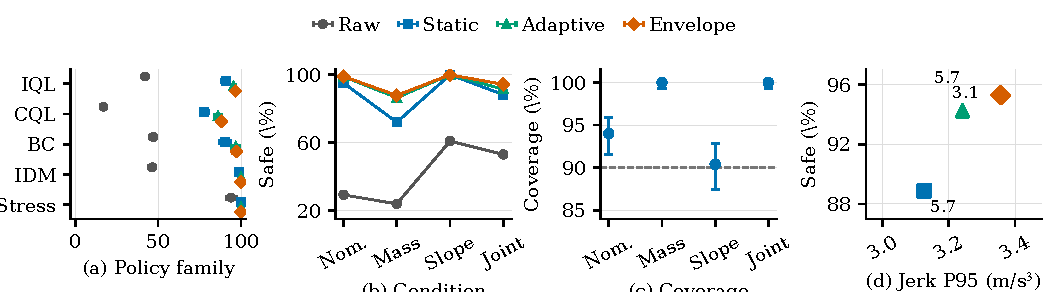
\includegraphics[width=\textwidth]{figures/fig2_evidence.pdf}
\caption{Compact evidence from ACC \emph{partial rollouts}. (a) Safety by
fixed policy family; intervals jointly resample shared reset trials.
(b) Safety across physical conditions. (c) Fresh one-step residual coverage
with exact 95\% binomial intervals; dashed line is $1-\alpha=0.9$.
(d) Safety versus comfort; point labels are mean warmed filter P95 latency
in ms. Projection rates are
6.51\%, 6.63\%, and 6.77\% for static, adaptive, and envelope filters.}
\label{fig:evidence}
\end{figure*}
\subsection{Policies, conditions, and evaluation protocol}
We evaluate four mixed-data IQL checkpoints, three mixed-data CQL checkpoints,
three independently bootstrapped linear behavior-cloning (BC) policies, an
intelligent driver model (IDM) expert, and a suboptimal-data CQL policy.
These 12 frozen policies cover
different learning objectives, training seeds, and data quality. Our real
ACC simulations are classified as \emph{partial rollout}: four conditions,
two lead-vehicle scenarios (braking and stop--go), 25 reset trials per
policy--condition--scenario cell, and a 500-step horizon. The four conditions
are $(m,\phi)=(1500,0),(1800,0),(1500,3),(1800,2)$ in kg and degrees.
All methods share initial physical states, seeds, and inference settings.
There are 2,400 paired policy--trial units and 200 distinct reset units across
the fixed policy suite.

The reduced model uses drag coefficient 0.24 and rolling coefficient 0.010,
compared with simulator values 0.30 and 0.012. The calibration model fixes
mass at 1500 kg and force gain at 0.7, using the observed grade; true force
gain is 1.0. The filter receives physical state, and the policy receives the
original normalized observation. The eight hypotheses combine
masses $\{1500,1800\}$, grades $\{0,3\}$, and force gains
$\{0.7,1.0\}$. Static and adaptive RACF use $q_\alpha=0.09188$,
obtained from the first 500 nominal calibration transitions with
$\alpha=0.1$ and $k=451$; the envelope filter uses $B=0.45$.
All three use $\eta=1$. Sequential quadratic programming solves each
projection. All data, models, and finite hypotheses are pre-generated local
assets; no external dataset enters these results. The openACC commercial
car-following database \cite{makridis2021openacc} is a natural source of future
lead-trajectory and external-coverage tests. All 12 selected checkpoints remain
frozen during evaluation.

The primary endpoint is an episode with no post-action ACC safety violation;
collisions terminate an episode. We report intervention and fallback
fractions, speed and gap RMSE, jerk P95, and warmed latency. Following
statistical guidance for RL evaluation \cite{agarwal2021precipice},
we resample reset trials jointly across policies within each
condition--scenario stratum (4,000 bootstrap draws). These intervals describe
the fixed policy suite. Exact McNemar tests \cite{mcnemar1947} compare
raw and filtered outcomes within each policy-specific cell, with Holm
correction over 288 comparisons \cite{holm1979}; the reanalysis is post hoc.
Paired intervals preserve the same resampled units \cite{efron1993}.

\begin{table}[t]
\caption{Episode-safe counts out of 600 per operating condition.
Coll. counts collisions across all 2,400 episodes per method.}
\label{tab:safety}
\centering
\setlength{\tabcolsep}{4pt}
\begin{tabular}{lrrrrr}
\toprule
Method & Nom. & Mass & Slope & Joint & Coll. \\
\midrule
Raw & 175 & 143 & 365 & 318 & 904 \\
Static & 571 & 432 & 600 & 530 & 0 \\
Adaptive & 594 & 519 & 600 & 549 & 0 \\
Envelope & 594 & 527 & 600 & 566 & 0 \\
\bottomrule
\end{tabular}

\end{table}

\subsection{Cross-policy safety and intervention}
Table~\ref{tab:safety} shows an increase from 1,001/2,400 safe raw episodes
to 2,133 static, 2,262 adaptive, and 2,287 envelope-filtered episodes.
All filtered runs complete 500 steps with zero collisions, compared with
904 collisions for raw policies. The paired safety gains are 47.17,
52.54, and 53.58 percentage points; the corresponding reset-cluster 95\%
intervals are [45.29,49.00], [51.04,54.04], and [52.21,54.96].
Across the 288 policy-specific comparisons, 149 remain significant after
Holm correction. Figure~\ref{fig:evidence}(a) shows the underlying heterogeneity:
IQL improves from 42.0\% safe episodes to 90.8--96.8\%, whereas CQL
improves from 17.0\% to 77.8--88.2\%. The suboptimal-data CQL policy
already reaches 94.0\% raw safety. Training-data quality therefore does not
by itself determine constraint pressure; the learned behavior matters.

The gains also appear in violation duration. Mean within-episode violation
fractions fall from 17.97\% for raw policies to 0.214\%, 0.122\%, and
0.095\% for static, adaptive, and envelope filtering. In nominal braking,
raw policies average 49.37 violating steps per episode, versus 0.03 for
static and zero for the other filters. Intervention is relatively sparse:
6.51\%, 6.63\%, and 6.77\% of actions are projected. Fallback occurs
on 0.91\%, 0.95\%, and 0.97\% of steps, respectively.
The envelope has 154 fewer unsafe episodes than static RACF while increasing
the projection fraction by 0.26 percentage points. These comparisons
measure operating-point effects; a margin-matched ablation is needed to
isolate the benefit of episode-level calibration itself.

\subsection{Independent coverage and control cost}
We separately evaluate one-step scores using 500 independent cruise resets
per condition, random actions, and zero to fifty random warm-up steps.
The threshold remains fixed at the value used in the closed-loop study.
The new reset seeds are disjoint from calibration and control evaluation,
and no transition duplicates any archived calibration or test record.
Coverage is 470/500 nominal (94.0\%, exact 95\% interval
[91.55,95.92]), 500/500 mass shift ([99.26,100]),
452/500 slope shift (90.4\%, [87.47,92.84]), and 500/500 joint shift
([99.26,100]); Fig.~\ref{fig:evidence}(c) summarizes these intervals. This
probe uses newly disjoint data after an audit of the
archived calibration/test split. Physical shifts can contract the residual
distribution, explaining the high mass-shift coverage.

\begin{table}[t]
\caption{Control performance on the 1,496 paired episodes where all four
methods complete 500 steps. Speed/gap: RMSE in m/s and m; jerk: mean
episode P95 in m/s$^3$; return: accumulated reward.}
\label{tab:utility}
\centering
\setlength{\tabcolsep}{5pt}
\begin{tabular}{lrrrr}
\toprule
Method & Speed & Gap & Jerk & Return \\
\midrule
Raw & 6.25 & 38.57 & 0.71 & -4934 \\
Static & 6.28 & 38.83 & 0.96 & -4624 \\
Adaptive & 6.28 & 38.85 & 1.15 & -4626 \\
Envelope & 6.28 & 38.88 & 1.24 & -4628 \\
\bottomrule
\end{tabular}

\end{table}

Raw collisions shorten the accumulation of predominantly negative rewards.
Consequently, the all-episode returns ($-4419$ raw versus approximately
$-5080$ filtered) combine performance and survival duration.
Table~\ref{tab:utility} adds a common-horizon comparison. On these paired
survivors, filtered returns improve from $-4934$ to approximately $-4626$,
while speed RMSE changes from 6.25 to 6.28 m/s. Comfort remains the
clearest cost: jerk P95 increases from 0.71 to 0.96--1.24 m/s$^3$.
This subset is a descriptive control-cost diagnostic; the full sample
remains the basis for safety reporting.



\subsection{Runtime and baseline diagnostics}
Evaluation uses four RTX 4090 GPUs for neural-policy inference and CPU
optimization for the filters. Figure~\ref{fig:evidence}(d) connects warmed
P95 latency to safety and jerk. Static, adaptive, and envelope filter P95s
are 5.72, 3.10, and 5.67 ms; their end-to-end P95s, including policy
inference, update, and environment step, are 6.07, 3.72, and 6.02 ms.
Candidate selection reduces the optimization workload in the adaptive
variant, whose update cost averages 0.25 ms. The filter P99s rise to
21.35, 11.13, and 22.28 ms, motivating explicit tail-latency measurement
when selecting a control period.

An independently implemented 20-step linear MPC provides a diagnostic
reference. Its OSQP solver \cite{osqp2020} uses constant lead-speed prediction
and soft headway constraints. Replaying the 200 distinct reset units
reproduces every recorded safety outcome; clipped force/action mapping
error stays below $1.49\times10^{-4}$ N. All 100,000 solver calls return
solved or solved-inaccurate status. MPC has zero collisions but violates
headway in every episode, illustrating the effect of lead braking on a
controller operating near the constraint boundary. Its action difference
from the learned policy is a controller deviation, so it is excluded from
the filter-intervention comparison.

\section{Discussion and Conclusion}
RACF connects residual calibration to robust correction of frozen RL actions.
Across 12 policies, the ACC evaluation shows substantial safety improvement,
policy-dependent constraint pressure, and a persistent comfort cost. Candidate
adaptation reduces latency; the fixed envelope achieves the highest measured
safety in this policy suite.

The current CTH margin changes with ego speed but omits closing-speed and
braking risk. A policy-conditioned sequential calibrator coupled to a dynamic
braking-aware margin is the next method step. Closed-loop guarantees further
require applied-action residual coverage and feasibility. Matched-intervention
comparisons across control tasks will test whether the safety gain persists
with lower jerk.

\clearpage
\bibliographystyle{IEEEbib}
\bibliography{references_rl}
\end{document}
